\section{Teoretický úvod}
  \indent\indent
  IO555 je masově vyráběný integrovaný obvod navržený v roce 1970 švýcarským inženýrem Hansem R. Camenzindem, který se nejčastej používá jako generátor nebo časovač. Na trh byl přivedn americkou firmou Signetics.
  
  \subsection{Vnitřní zapojení}
    \indent\indent
    Uvnitř obvodu je pět rezistorů o hodnotě $5~k\Omega$, dva komparátory, klopný obdov RS, Invertor a bipolární tranzistor NPN a rezistor omezující prodou do báze tohoto tranzistoru.
    
    \begin{figure}[H]
    \centering
    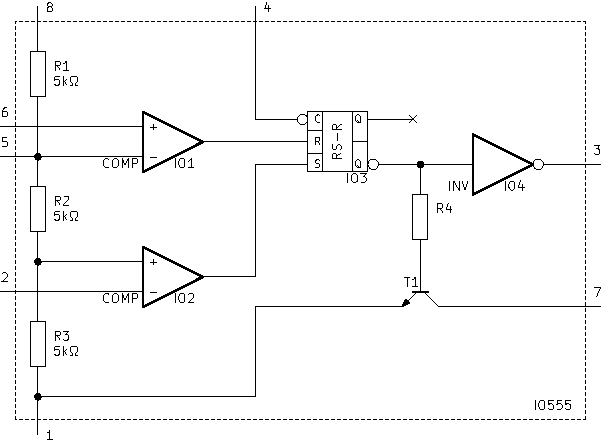
\includegraphics[width=15cm]{../img/sch1.pdf}
    \caption{Vnitřní zapojení IO555}
    \label{sch:1}
  \end{figure}
    
  \subsection{Princim činnosti IO555}
    \indent\indent
    Obvod ke své funkci vyžaduje napětí mezi piny 8 a 3 a to v rozmezí $4,5-16~V$ pokud se jedná o typ NE555, SA555, SE555C, typ SE555 pracuje s napetím v zozsahu $4,5-18~V$. Protože je napětí přivedeno na dělič, který se skládá s pěti totožných rezistorů, tak se zizdělí na tři torožné úbytky. Mezi piny 8 a 1 je napětí rovno $\frac{3}{3}U_{CC}$, mezi piny 5 a 1 je rovno $\frac{2}{3}U_{CC}$ a meti neinvertujícím vstupem komparítoru IO2 a pinem 1 je rovno $\frac{1}{3}U_{CC}$. Bistabilní klopný obvod RS vydohnocuje výstupy komparátorů, pokud není na pinu 4 úroveň L, která by bistabilní klopný obvad RS držela v resetu. Podmínky pro výstupy komparátorů v úrovních H:
    
    Pro komparátor IO1:
    \begin{eqnarray}
      U_{P6} - \dfrac{2}{3} \cdot U_{CC} &>& 0 \nonumber\\
      U_{P6} &>& \dfrac{2}{3} \cdot U_{CC}
    \end{eqnarray}
    
    \hspace*{2cm}kde:\newline    
    \hspace*{4cm}$U_{CC}$ \dotfill napětí mezi piny 8 a 1\hspace*{4cm}\newline
    \hspace*{4cm}$U_{P6}$ \dotfill napětí mezi piny 6 a 1\hspace*{4cm}\newline
    
    Pro komparátor IO2:
    \begin{eqnarray}
      \dfrac{1}{3} \cdot U_{CC} - U_{P2} &>& 0 \nonumber\\
      U_{P2} &<& \dfrac{1}{3} \cdot U_{CC}
    \end{eqnarray}
    
    \hspace*{2cm}kde:\newline    
    \hspace*{4cm}$U_{CC}$ \dotfill napětí mezi piny 8 a 1\hspace*{4cm}\newline
    \hspace*{4cm}$U_{P2}$ \dotfill napětí mezi piny 2 a 1\hspace*{4cm}\newline
    
    
    Pokud bude výstup komparátoru IO1 v úrovni H, tak se otevře tranzistor T$_1$ a na pinu 3 bude úrověň L. Pokud bude výsup komparátoru IO2 v úrovni H, tak se tranzisto T$_1$ zavře a na pinu 3 bude úroveň H.
   
  
